\documentclass[12pt]{article}

%USEPACKAGES
\usepackage[margin=2.5cm]{geometry} % Change border margins.
\usepackage[titles]{tocloft} % Table of Contents, manual add.
%\usepackage{mcode} % Load matlab code into LaTeX.
\usepackage[parfill]{parskip} % Removes indents
\usepackage[hidelinks]{hyperref} % Clickable links in PDF.
\usepackage{fancyhdr}
\usepackage{graphicx}
\usepackage{epstopdf}
\usepackage{float}
\usepackage{amsmath,amssymb,amsthm,multirow,algorithm,algorithmic,amsfonts}
%\usepackage{gensymb}
%\usepackage[square,numbers,comma,sort&compress]{natbib}
\usepackage[titletoc]{appendix}
\usepackage[final]{pdfpages}
\usepackage{afterpage}
%\usepackage{mdwlist} % Compact lists (itemize*)
\usepackage{fixltx2e}
%\usepackage[table]{xcolor}
%\usepackage{expl3}

\usepackage{lscape}
\usepackage{rotating}

% PAGESTYLE
\pagestyle{plain}

% COMMANDS
\newcommand{\HRule}{\rule{\linewidth}{0.04cm}}
\renewcommand{\abstractname}{{\Large Summary}}
\renewcommand{\cftsecleader}{\cftdotfill{\cftdotsep}}
\setlength{\parskip}{12pt plus8pt minus6pt}

% ENVIRONMENTS
\newenvironment{drawing}


%\title{\textbf{AE3200 - DSE-02 Controlable Inflatible Aeroshall \\ \smallskip Logbook}}
%\date{\today}
%\author{Lucas Mathijssen}



\begin{document}
\clearpage
\thispagestyle{empty}

\begin{center}

%Upper part of the page
\textsc{\LARGE Delft University of Technology}\\[0.3cm]
\textsc{\Large Design Synthesis Exercise}\\[0.5cm]

%Title
\HRule \\[0.4cm]
{\Large \bfseries Design of a Controllable Inflatable Aeroshell}\\[0.2cm]
{\Huge \bfseries Logbook}\\[0.2cm]
\HRule \\[1.2cm]

\vspace{10mm}
Lucas Mathijssen
\\
\today
\\
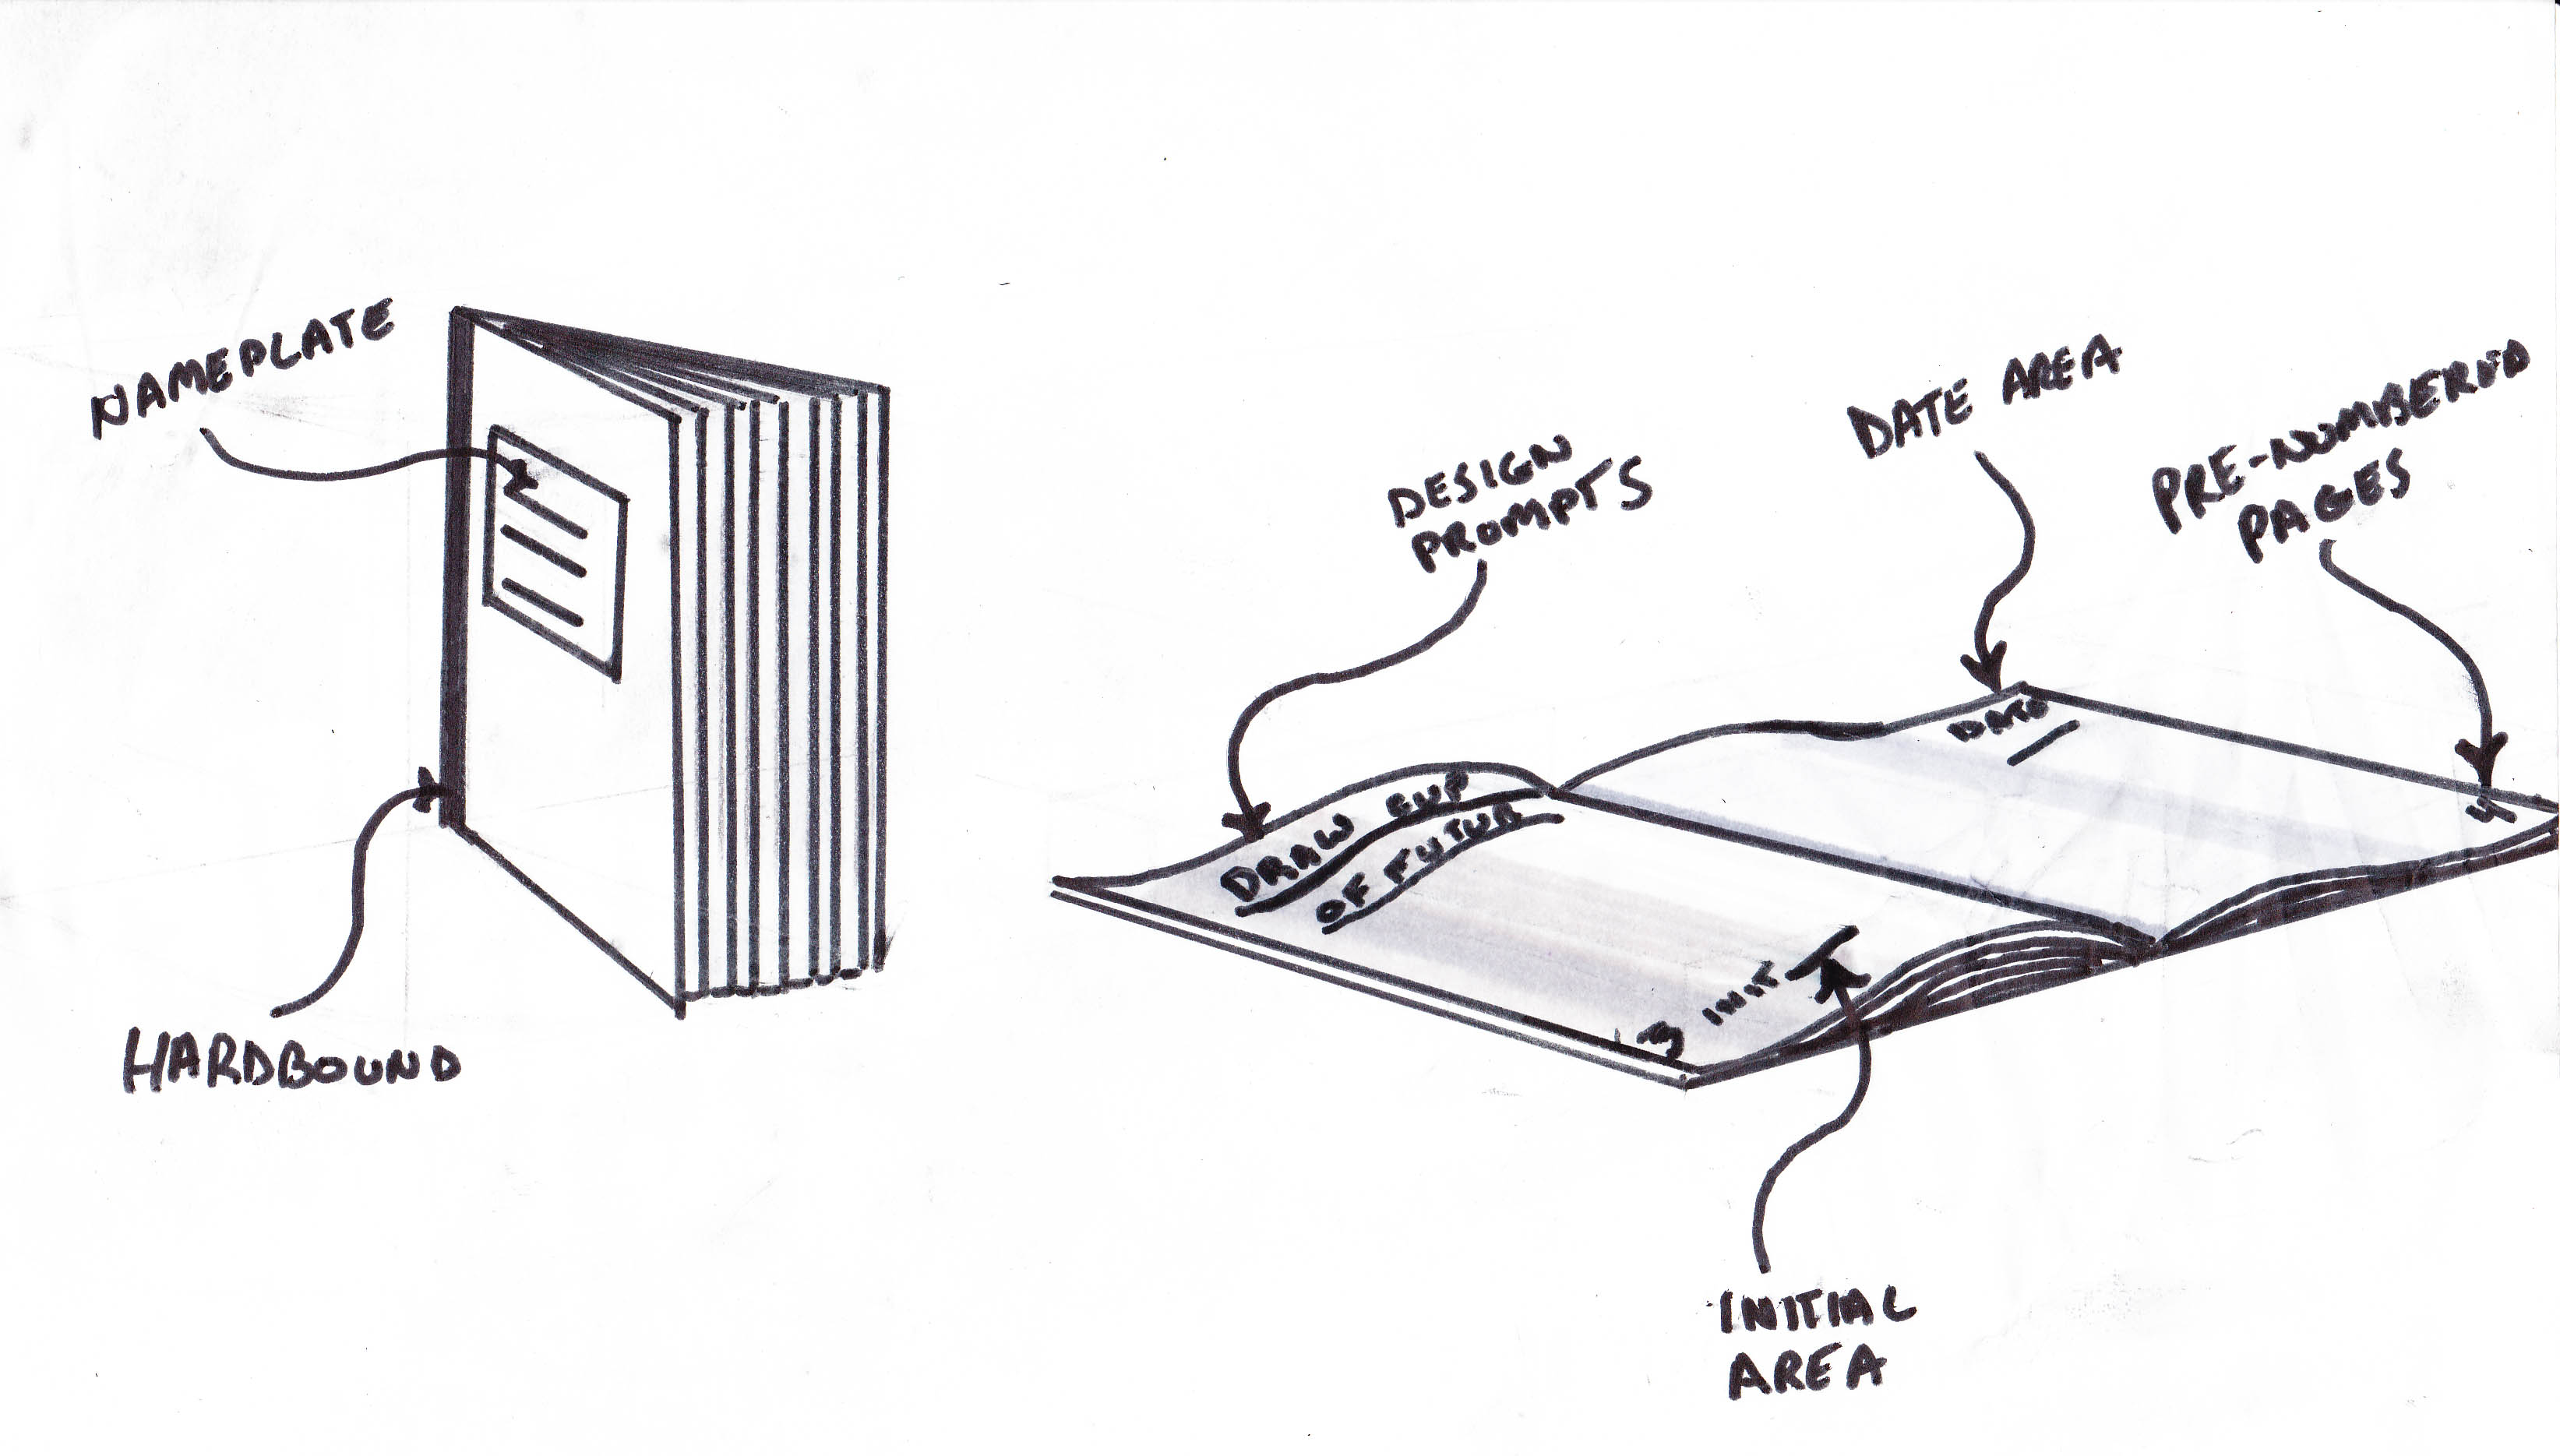
\includegraphics[width=16cm]{Figures/notebooksketch.jpg}

\end{center}


%Table of contents
\newpage
\pagenumbering{roman}
\tableofcontents


%Chapters
\newpage
\pagenumbering{arabic}
\newpage
\section{Schedule}

\newpage
\section{Reviews Viewgraph Hardcopies}
\newpage
\section{Minutes of Status Meetings}
In this section all minutes of the status meetings will be archived. For these minutes, Abbreviation will be used for the speakers. the abrivations can be found in table \ref{tab:Abb} below.

\begin{table}[H]
	\caption {Abbreviations of names}
	\centering
    \begin{tabular}{|l|l|}
    \hline
    Abbreviation for person & Full name      \\ \hline
    HD                      & Herman Damveld \\ \hline
    NR                      & Niels Reurings \\ \hline
    DD                      & Dennis Dolkens \\ \hline
    J                       & Joost          \\ \hline
    L                       & Lucas          \\ \hline
    A                       & Alexander      \\ \hline
    G                       & Guido          \\ \hline
    D                       & Dawud          \\ \hline
    Se                      & Sebastiaan     \\ \hline
    B                       & Bj\"{o}rn      \\ \hline
    Su                      & Suthes         \\ \hline
    T                       & Twan           \\ \hline
    \end{tabular}
    \label{tab:Abb}
\end{table}

%\subsection{Kick-off, 20-04-2015 9:00}


\subsection{Status Meeting 1, 22-04-2015 14:00}
Location: Fellowship Meeting room 1\\
Time: Joost opened the meeting at 14:00\\
SECRET CODE1: yes, there is a secret code

\subsubsection{Agenda}
J: Add a set of questions between points 5 and 6 in the agenda.\\
J: Additional question: Should the communication be in English or in Dutch? 
HD: As long as there is no external or formal communication, Dutch communication may be used.

\subsubsection{Organizational task devision}
D: task division is as is shown in table \ref{tab:tasks}, where the left part of the table describes the distribution of the general work division, while the right columns describe the technical task division.

\begin{table}[H]
	\caption {Task distribution}
    \begin{tabular}{|p{0.25\textwidth}|p{0.2\textwidth}|p{0.25\textwidth}|p{0.2\textwidth}|}
    \hline
    General task division                 & Names      & Technical task devision & Names                    \\ \hline \hline
    Chairman (CH)                         & Joost      & Structures              & Bj\"{o}rn; Alexander         \\ \hline
    Secretary (S)                         & Lucas      & Aerodynamics            & Guido; Joost; Sebastiaan \\ \hline
    Planning (Pl)                         & Alexander  & Thermodynamics                 & Suthes; Lucas            \\ \hline
    Systems Engineer (SE)                 & Guido      & Control                 & Dawus; Twan              \\ \hline
    Documentation and Archiving ( D \& A) & Dawud      & ~                       & ~                        \\ \hline
    Risk manager (YOLO)                   & Sebastiaan & ~                       & ~                        \\ \hline
    Editor (Ed)                           & Bj\"{o}rn      & ~                       & ~                        \\ \hline
    Verification (Ver)                    & Suthes     & ~                       & ~                        \\ \hline
    Validation (Val)                      & Twan       & ~                       & ~                        \\ \hline
    \end{tabular}
    \label{tab:tasks}
\end{table}

HD: You should make sure that you are able to switch between departments, because you cannot yet know how much work a department is going to have. It can be easy if you have people in multiple technical departments, such that there is not time loss in getting acquainted with a new topic if switching occurs.\\
G: As a SE I will be responsible for the overview and make sure that this will not be a problem.\\
HD: And who is the person that keeps a clear overview of the latest parameter numbers? Make sure that there is a clear description of the tasks and that no work is left undone. You can for instance keep the parameter values in an excel sheet.\\
L: We could also keep the latest variables as an input file in MATLAB, that runs our tools. \\
NR: Then keep in mind that you need time logs, such that there is no confusion about changes in the input by a person.\\

\subsubsection{upcomming deadlines}
J: We moved the deadline for the baseline review to may 1st, because of the free days after the weekend must be free and not used for checking. \\
HD: OK.\\
L: Since our project plan is almost finished, can we send the report today, so that you can check it tomorrow? In that way we can discuss it on Friday and we will still have time to correct the last things.\\
HD: I don't have much time. I can see what I can do.
NR \& DD: We can have a look. If you can get an advantage this way, I would seartenly make use of it if I were you.\\

\subsubsection{Questions}
Q1: \textit{L: The requirements state that the tutor and coaches should always be able to look at the latest version of the logbook, how shall we realise this?}\\
HD: We can use any cloud storage, but I would prefer If you have a look at 'surfspot'.\\
L: What should we put on the storage cloud?\\
HD: General deliverables, like the logbook, agendas and deliverables. No large datasets. Also note that you need to print certain things. \\

Q2: \textit{Se: How detailed should the risk mitigation plan be?}\\
HD: For the baseline review the risk should be evaluated very generally. We want to see that the group understands the requirements and what the driving requirements will be. cost for example is not a requirement and hence it shouldn't be elaborated extensively, otherwise you did something wrong. Also, You don't have to write a plan for the complete mission, you must focus on the re-entry. You don't have to design the capsule, you can find data on this from similar missions. Examples are the Orion and Apollo mission from NASA.\\

Q3: \textit{L:What is the starting point of the mission, will we start at launch or in the atmosphere, or somewhere in between?}\\
HD: In general, the begin point of your mission is a speed of 7 km/s at an altitude I will provide you with on a late time.\\
D: What about the orientation, is that free to choose?\\
HD: You will see that there are only few options for a human flight to land on mars, so this will automatically provide you with a requirement.\\

Q4: \textit{Su: How detailed should the sustainability part be, since it will determine 10\% of our symposium grade?}\\
HD: This is not a very important part in the design, because we cannot bring extra mass just for the use of sustainable materials. This will induce a large snowball effect, such that more propellant is needed. Burning more propellant is not at all sustainable. \\
NR: You can focus on things like space debris, materials used and how they are produced.\\
DD: Or on life forms that you will bring to space that might cause damage, etc.\\
HD: So in general, don't underestimate it. Treat it with respect, but don't make it a large part of your design.\\

Q5:\textit{L: We had some problems with the code for the requirements, but it is solved now}\\
HD: Now I am curious.\\
L:described the code: Mission-Concept-number-subsystem-number.\\
NR: It's nice that you did it, but a bit a waste of your energy.\\
HD: By the way, you don't need two concepts in the end. That's something we did two years ago with the same project, but I wanted to remove it from the project this time. I must have forgotten it. So after the mid-term review, you have to consider only one design.\\

\subsubsection{W.F.C.T.T.T}
No comments
SECRET CODE2: It's raining meatballs

\subsubsection{Survey}
A:-\\ 
B:-\\
Su:-\\
D:-\\
\textit{NR: For the editor, it might be very stressful to do proofreading, because a lot of people might submit their parts last minute, don't you want more than one person in this department?} \\
B: The task division only states final responsibility, but overall more than one person will work on this.\\
T:-\\
Se:-\\
\textit{J: I am a literature study right now and I see that a lot of questions in the literature are not solved yet, how should we proceed with this?}\\
HD: You should only focus on your own design, but I want to make the problem a bit broader than it is. I want you to think of other concepts than only aero shells. You need to incorporate this in your design option tree.\\
T: So should our mission statement change? Because we have stated that we will only look at aero shells.
HD: No, I just want you to apply broader knowledge during the concept development, such that you will get a better understanding of the mission.\\
\textit{G: Should we also design the landing, or where will our mission end?}\\
HD: No, that is outside the scope of this exercise. I will later send you a final altitude with a corresponding speed that will indicate the end of your mission.\\

HD: Yesterday I had contact with a very smart student who did this same project two years ago. He indicated that he was willing to help you with questions about the project. I will later send you his name and contact information. If I were you, I would not refuse this offer.\\

\subsubsection{Adjournment}
The next meeting will be Friday 24-04-2014 at 10:00 in Meeting room 1.\\

Adjournment at 15:00

\subsection{Status Meeting 2, 24-04-2015 14:00}
\subsubsection{Call to order}
Locatie: Fellowship Meeting room 1\\
tijd: Joost opened the meeting at 14:00\\

\subsubsection{Agenda}
J: Ik wil tussen puntje twee en drie nog een kopje voor het goedkeuren van de notulen toevoegen.\\

\subsubsection{Acceptance of minutes}
De notulen zijn door iedereen goed gelezen, bravo.\\

N: Mijn naam is verkeerd gespeld in de notulen, het is namelijk Reurings en niet Reuring. Dit staat volgens mij ook fout in de reader. Maar verder is het wel goed.\\

L: Ik zal het aanpassen.\\

\subsubsection{Review of Project Plan}
HD: Jullie hebben het werk mooi op tijd ingeleverd. Dat is goed, want met een goed project plan valt of staat een project.\\

J: We hebben het rapport van te voren ingeleverd. Hebben jullie nog opmerkingen over het verslag die wij kunnen doorvoeren?\\

HD: Ik heb naar het verslag gekeken en ik heb nog een paar puntjes.\\
\textit{1: HD: De preface, nou nou.. dit ziet er een beetje uit als slijmen naar de begeleider. Als klant zit ik hier niet echt op te wachten. houd het vooral zakelijk.}\\

\textit{2: HD: In de introduction bij de purpose of the project plan geven jullie aan een general approach te hebben. maar dit project is juist heel specifiek, daar stoorde ik mij aan.}\\
Su: Het gaat eigenlijk meer over onze aanpak van dit project.\\
HD: Zou je bij het ontwerpen van een reactor het zelfde plan van aanpak hebben? Ik hoop het niet!\\
T: Wat Suthes bedoeld is dat het gaat over het al omvattende plan binnen dit specifieke onderwerp.\\

ZOEKWOORD: STRAWMAN CONCEPT\\

\textit{3: HD: De objective statement geeft wel heel specifiek aan dat er gebruik gemaakt moet worden van bestaande launchers, dit trekt de aandacht weg van het eigenlijke doel.}\\
L: Dit is om duidelijk aan onze klant aan te geven wat wel en niet binnen onze taakomschrijving valt.\\
HD: En andere requirements niet? dan zou je ze er allemaal in moeten steken.\\
NR: Zorg dat je statement SMART is (Specific Measurable Attainable Realistic and Time dependent).\\

\textit{4: NR: Er missen in die sectie ook referenties. zo staat er bijvoorbeeld een hele mooie mission tabel, maar er staat nergens een referentie waar de data vandaan komt.}\\
T: Die staat geloof ik wel ergens in de tekst.
HD: Wees secuur! het is hier niet helemaal duidelijk. \\
NR: Wees er zelf erg bewust van wat je opschrijft, niet verwijzen wordt gezien als plagiaat en kan grote gevolgen hebben.\\
HD: dus elke keer als er een statement wordt gemaakt in je tekst zonder dat deze is uitgelegd, moet deze statement van jezelf komen of ergens anders vandaan komen. In het laatste geval is een echt referentie nodig! Wees er heel voorzichtig mee.\\

\textit{5: DD: jullie mission need statement is vreemd geformuleerd. Nu lijkt het alsof jullie zelf gaan demonstreren dat het werkt, hoewel jullie alleen maar het design verzorgen.}\\
All: We zullen het aanpassen.\\

\textit{6: DD: In section 2.1 staat ook ergens aircraft i.p.v. spcecraft}

\textit{7: HD: In section 2.2 begint jullie requirement code altijd met CIA en SYS, deze code is daardoor onnodig lang.}\\
L: Dat is zo geformuleerd omdat we eerst wouden werken met meerdere concepten, maar dat is nu niet meer nodig. Tevens staat CIA altijd aangegeven zodat de klant direct kan zien over welk project het gaat, van de vele projecten waarin hij of zij geïnvesteerd heeft. Ik zal het aanpassen.\\

\textit{8: HD: Requirement 5 is ook niet echt duidelijk}\\
A: Deze requirement is overgenomen uit de reader en is sowieso vaag.\\
HD: Wat was er niet duidelijk dan?\\
A: Ik snap niet waarom deze requirement zo beschreven is. de massa van de heat shield mag maar 10\% van het totale gewicht, waarbij het totale gewicht 10,000 kg is. Maar deze gewichten staan helemaal niet vast. Moeten de ene mee schuiven met de ander als de gewichten veranderen?\\
HD: Ja, dat klopt en die 10\% is een maximum gewicht. Ik hoor het graag als er geschoven moet worden met de requirement.\\
NR: Het uiteindelijke gewicht zal zijn hangt af van hoe het zich in de praktijk zal uitwijzen.\\
Hd: Het grote lijn idee is in ieder geval dat je voertuig aan het begin van de re-entry een gewicht van 10,000 kg heeft. Deze massa moet worden afgeremd.\\

\textit{9: HD: bij de OBS zie ik nergens een astrodynamics department?}\\
T: We hebben hierover nagedacht, dit valt onder de orbital- en control department.\\

\textit{10: NR: In de tekst staat niet goed beschreven wat Verification en Validation is. Weten jullie hoe en wat het is?}\\
T: Verification heeft meer met je eigen requirements te maken, hoewel validation meer over requirements van de customer gaat.\\
L: Zoals ik het zie gaat verification erover of je het product correct maakt en validation erover of het product wel de waarheid simuleert.\\
HD: Dit moeten jullie nog wel even aanpassen. Verification gaat over de vraag of je het goed doet en validation of je het goede doet.\\

\textit{11: HD: Ik zag ook dat er nog steeds maar een planner is en maar een persoon op systems engineering. Hier hebben we het vorige keer nog over gehad! Waarom is er niets veranderd?}
G: In principe werken we er met meer mensen aan, maar er is een eind verantwoordelijke.\\
DD: Op deze manier valt er wel heel veel verantwoordelijkheid op de SE. Zorg dat er goed ondersteuning is, die heb je nodig.\\
T: V\& V team geeft ook ondersteuning aan de SE. SE let erop of het gebeurt, V\& V of het wel goed gebeurt.\\
HD: En wat doet de planner als jullie je deadlines niet halen.\\
A: Het idee is dat we niet gaan achterlopen, daar is de planning voor.\\
NR: Hier moet je mee uitkijken, dit gaat sowieso wel gebeuren en als het gebeurt schuift het werk op en dat gaat altijd ten koste van het schrijfwerk. Dat zal de editor niet zo leuk vinden.\\
T: In principe moet de planner dan op tijd aan de bel trekken.\\
D: Ja, maar we moeten ook beschrijven hoe en wanneer.\\
A: Zo vroeg mogelijk.\\
NR: Dus jij houdt overzicht over de planning en stuurt dagelijks bij?\\
A:Ja, aan het einde van de dag, na onze group meeting.\\

\textit{12: HD: Over de WBS: Jullie hebben ook tijd ingeplant voor het ontwikkelen van tools, dat is heel goed! dat wordt vaak vergeten.}\\
NR: Ik vond het juist wel een beetje de andere kant opslaan. Er was wel veel tijd vrijgehouden voor tools, maar weinig tijd voor het daadwerkelijke design. De twee kunnen niet zonder elkaar.\\
DD: Gaan jullie alles zelf ontwikkelen?\\
D: Een combinatie van.\\
DD: Het lijkt nu inderdaad veel werk om de tools te ontwikkelen, waar je kunt uitbesteden zou ik uitbesteden.\\

\textit{13: HD: Ik merk dat jullie vaak wel weten wat jullie willen gaan doen, maar dat het niet duidelijk staat opgeschreven. Als dit in een keer duidelijk wordt gedaan scheelt het een hoop discussie tijd! (goede tip)}\\

\textit{14 NR: Ik zie ook niet zo goed waar de iteration in jullie design proces staan weergegeven.}\\
G: In het detailed design.\\

\textit{15: HD: Jullie workpackages in de WBS komen niet overeen met de workpackages in de Gantt-chart.}\\
B: Dat komt omdat de WBS vrij globaal is en de Gantt-chart niet. We volgen niet de workpackages omdat we zo beter kunnen schuiven in de gantt-chart als dat nodig blijkt.\\
HD: Het is gebruikelijk om wel de zelfde workpackages te hebben. Het moet naadloos in elkaar over kunnen lopen.\\

\textit{16: HD: Verder is er volgens mij inhoudelijk niets mis mee.}\\

\textit{17: NR: Bij sustainability moet je niet zeggen dat het niet belangrijk is als je er net een hele pagina aan hebt gewijd. Dan ben je jezelf aan het onderuit halen.}\\
DD: Er er miste ook COOSPAR.\\
Se: Zal het aanpassen.\\

\textit{18: NR: In je referentie lijst moet je wel schrijven of iets een thesis /journal of een article is, zodat ik weet ik moet benaderen als ik verdere informatie wil hebben.}\\
HD: Gebruiken jullie bibtech? weten jullie hoe dat werkt? Je kunt ook "mandolate" gebruiken voor het managen van je referenties, dan krijg je geen dubbele referenties in je lijst, etc. Dat werkt het beste uit mijn ervaring.\\
DD: Je kunt ook de bibtech code direct van google scholar halen.\\
D: Ik zal kijken of ik dat kan oplossen.\\

\textit{19: HD: Dit was veel kritiek, maar jullie hoeven niet te denken dat jullie het slecht hebben gedaan, inhoudelijk was er niets mis met het werk.}\\

J: Bedankt voor de feedback.\\


\subsubsection{Deliverables}
J:Er is een mismatch in de deliverable tabel. Op blackboard zijn er updates en het is niet duidelijk wat we nou moeten inleveren.\\
HD: Ja, ik heb het gezien, heel vervelend. Maar de tabel in de reader is leidend.\\

A: Over de baseline review. wat houdt het precies in? Ik zag dat we een agenda moeten voorbereiden, maar wat moet erin?\\
HD: Zoals we nu om de tafel hebben gezeten voor het project plan, zullen we tijdens de baseline review om de tafel gaan zitten voor jullie baseline report. Het is net iets formeler. Jullie moeten dan ook presenteren, niet iedereen, maar 3 tot 4 mensen (Uiteindelijk moet iedereen een keer gepresenteerd hebben). Jullie moeten ook zelf voor een zaal zorgen en jullie moeten er ook voor zorgen dat jullie goed voorbereid zijn. Hiermee bedoel ik dat de computer al klaar moet staan en dat jullie gelijk kunnen beginnen. Daar beoordelen we jullie op.\\
J: Is er een pagina limiet voor de baselinereview?\\
HD: Blijf ongeveer onder de 50 pagina's.

L: Over het logbook. Dat staat nergens als een deliverable, maar het is wel een officieel document, hoe zit dat?\\
HD: Jullie hoeven het niet in te leveren, maar ik wil het wel in kunnen zien voor het geval er iets fout is gegaan, omdat het design proces hier in is vast gelegd samen met alle belangrijke beslissingen etc..\\

\subsubsection{Questions}
\textit{Q1: B: Over de geometrie van ons voertuig. moeten we ook voor de payload ontwerpen?}\\
HD: In principe moet je ook je payload designen. Als je dit niet weet kan dat later een groot sneeuwbaleffect veroorzaken.\\

\textit{Q2: G: Ik vraag me af waar onze missie eindigt en met name over welke orde van grootte dit gaat. In andere woorden, moeten we ook ontwerpen voor het subsone regime?}\\
HD: Nee, dan is jullie missie al afgelopen. Jullie hoeven enkel te ontwerpen voor de hypersone vlucht.\\

\subsubsection{W.F.C.T.T.T}
L: Een vriendin van mij zit in een ander DSE groepje, en zij willen graag ook gebruik maken van MARS-Gram, kan dat?\\
HD: Dat is goed, maar onder bepaalde voorwaarden. Ik heb van NASA goedkeuring gekregen voor het gebruik binnen de DSE, maar het programma mag daarbuiten niet gebruikt worden.\\

\subsubsection{Survey}
\textit{DD: Hebben jullie de Belbin test nog gemaakt? Wat was het resultaat?}\\
T: We hebben de test gedaan en we hebben van bijna alle karakters wel iemand, behalve twee karakters geloof ik.\\
D: We kunnen het resultaat wel doorsturen.\\
HD: Pas op, dit kan een valkuil zijn. ga niet alleen focussen op de taken waar je goed in bent, maar doe alles wat nodig is.\\

\subsubsection{Adjournment}
De volgende vergadering zal plaatsvinden op 29-04-2015 om 16:00 in meeting room 2.\\

Joost sluit de vergadering om 11:24. iedereen is zeer opgelucht.\\


\subsection{Status Meeting 3, 29-04-2015 16:00}
\subsubsection{Call to order}
Locatie: Fellowship Meeting room 2\\
tijd: Joost opened the meeting at 16:01\\


\subsubsection{Agenda}
J: Ik wil tussen puntje twee en drie nog een kopje voor het goedkeuren van de notulen toevoegen. Volgende keer staat die er standaard in.\\

\subsubsection{Acceptance of minutes}
G: Bij het antwoord op mijn vraag over het snelheidsregime waarin we moeten ontwerpen miste dat we ook voor supersoon moeten ontwerpen.\\
L:Ik zal het aanpassen.\\

\subsubsection{Action points}
J: Een action van de vorige vergadering was het afmaken van het verbeterde project plan. Is dit naar tevredenheid gebeurt?\\
HD: Ik wist niet dat jullie hier verder commentaar op wouden hebben.\\
J: Ik vraag het meer omdat het vorige keer een action Item was.\\
HD: Ik heb het diagonaal doorgelezen en ik zag dat de veranderingen waren toegepast, verder heb ik geen commentaar.\\
DD: Ik heb mijn deel nog eens doorgelezen en alles was gewoon doorgevoerd, dus het is wel goed. Maar ik zag nog wel een typefoutje in de mission statement. en er was ook een foutje in de lay-out waarbij tekst door een tabel heen liep.\\

\subsubsection{Requirments}
\textit{Q1: T: met betrekking tot de g-loads, mag je 3 aardse g's in elke richting trekken of alleen in een richting?}\\
HD: Het gaat om de lengte van de vector, dus in een richting. Als de astronauten voor 10 dagen lang meer dan 3 g moeten dragen vinden ze dat niet fijn.\\
Se: We kunnen wel een budget maken over de tijd van de gehele missie, zodat we rekening kunnen houden met eventuele groei.\\
HD: Nee, dat is niet de bedoeling.

\textit{Q2: T: En hoe zit het met peak g loads?}\\
G: Moeten we ons altijd aan de 3 g requirement of we voor korte tijd ook meer g's dragen?
HD: In principe moet je gewoon ontwerpen voor de 3 g requirement, maar ik ben als klant wel geïnteresseerd in andere opties. Als jullie met een bepaalde trajectory komen die over het algemeen veel beter is maar wel heel even wat hogere g's moet kunnen hebben dan heb ik daar wel oor voor. Maar, het moet geen onderhandel punt worden, nogmaals, het is in principe de bedoeling dat je voor 3 g requirement ontwerpt.


\subsubsection{Survey}
\textit{Q1: Se: Ik heb een familie situatie en het zou kunnen zijn dat ik binnenkort wat uren ga missen. Wat is uw beleid hierin? Ik wil in principe wel gewoon mijn uren goed maken.}\\
HD: Shit happens. Kijk, daar kunnen we gewoon mee omgaan. Weg blijven moet alleen geen excuus worden om je werk niet te doen. Ik zeg niet dat het zo is, maar houdt er rekening mee. Ik had twee jaar geleden een DSE groepje waarbij iemand mazelen had en thuis moest blijven en dat hebben we prima kunnen regelen via Skype, dus er is altijd wel een oplossing te vinden. Je moet wel altijd laten weten aan Joris Melkert dat je weg bent, want hij is hier nogal streng in. Hij hoort dit soort dingen ook graag van te voren. Daarnaast moeten team members niet gewoon het werk van de persoon opvangen die weg gaat, maar het aankaarten als dat nodig is.\\

\textit{Q2: J: Ik had nog een mailtje gestuurd over MARS-Gram, maar misschien kunnen we dat zo oplossen.}\\
HD: Daar kunnen we na de meeting nog wel samen naar kijken.\\

\textit{Q3: L: Over het thermodynamica gedeelte van de literatuur studie, hoe diep moeten we dat nu uitzoeken? want het wordt of vrij makkelijk of juist veel te moeilijk. Ik weet echt nog niet hoe ik bijvoorbeeld een berekening kan maken van materiaal wat zichzelf aan het opofferen is, omdat de boundary conditions gewoon veranderen.}\\
HD: Zo veel detail is nu nog echt niet nodig. Je zou nu heel oppervlakkig moeten weten wat voor componenten er zijn en hoe het design beperkt wordt. Later komen de heftige berekeningen nog wel.\\
HD: Het is ook wel het geval met deze DSE opdracht dat het niet zo een twee drie het boekje volgen is. Je kunt niet even de bibliotheek inlopen en het juiste design punt opzoeken in bijvoorbeeld een Raymer boek. Je moet zelf echt een beetje gaan nadenken over het ontwerp.\\
L: Dus het is een beetje de jazz onder de DSE opdrachten?\\
HD: Hoe bedoel je? Daar houd ook niemand van?\\
L: Nee, in de zin dat je zelf moet improviseren en niet zomaar het boekje kunt volgen.\\
NR: Ik ben zelf bezig geweest met high temperature composites en ik kan je wel een tip geven. Niet alleen het materiaal kan een aanduiding geven van je thermal protection, maar ook de plaats kan een indicatie geven. denk aan de tegels op de space shuttle.\\

Zoekwoord: Requirements\\

\subsubsection{W.F.C.T.T.T}
HD: Hoe staat het met de planning? Hebben jullie een beetje het idee dat jullie op stoom zijn gekomen?\\
Allen: Ja hoor.\\
L: Ja, zeker na de literatuur studie, dan krijgt de opdracht steeds meer een bepaalde vorm.\\
T: We zijn gewoon lekker bezig en soms zie je mensen ook een eureka moment krijgen. 'OO, zo zit dat in elkaar' hoor je ze dan denken.\\

NR: Tijdens jullie dagelijkse meeting, bespreken jullie dan ook wat er inhoudelijk is gebeurt?\\
T: Ja, dat bespreken we.\\
NR: Houden jullie ook rekening dat jullie moeten gaan presenteren en ook nog een presentatie moeten maken?\\
T: Ja, dat staat ook in onze planning.

\subsubsection{Survey}
Er zijn geen verdere vragen

\subsubsection{Adjournment}
De volgende vergadering zal plaatsvinden op 01-05-2015 om 10:30 in meeting room 2.\\

Joost sluit de vergadering om 16:24.\\


\subsection{Status Meeting 4, 01-05-2015 10:30}
\subsubsection{Call to order}
Locatie: Fellowship Meeting room 2\\
Aanwezig: HD, NR, DD, J, L, G, A, B, T, D, Su, Se\\
Verontschuldigd: - \\
Afwezig: - \\
tijd: Joost opent de vergadering om 10:31\\

\subsubsection{Agenda}
De dagorde wordt goedgekeurd\\

\subsubsection{Acceptance of minutes}
HD geeft aan dat de notulen zakelijker moet worden geschreven, na het zien van een ontwikkeling over de voorgaande notulen. L gaf aan dat dit is gebeurt om de notulen interessanter te maken, maar zal het aanpassen.\\

\subsubsection{Questions}
\textit{Q1: J: Er is een requirement over de reliability van het control systeem, maar wat houdt het control systeem dan in?}\\
Er volgt een interessante discussie over de reliability van een subsysteem. Er wordt geconcludeerd dat de reliability van een subsysteem wordt gebruikt om de functionaliteit vast te leggen en dat zij volgt uit de reliability van het totale systeem. Specifiek voor het control subsysteem geldt dat de reliabiltity afhangt van de huidige technologie evenals een iteratief process tussen external loads, thermal loads en het control subsysteem.\\

\textit{Q2: Se: Welke elementen moeten er in een risk map, aangezien het een levend document is en we nog in een vroeg stadium zitten}\\
HD geeft aan dat er nog niet veel in moet staan omdat het project nog in een vroeg stadium verkeerd, waardoor nog niet veel bekend is over subsystemen. NR voegt hieraan toe dat het nu vooral een handige tool is om key-aspacts te vinden die later in het proces veel werk uren zullen vergen.\\

\subsubsection{W.F.C.T.T.T}
HD vraagt of iemand zijn ringmap heeft gevonden. Dit was niet het geval.\\

J geeft aan dat MARS-Gram nu wel werkt.\\ 
\subsubsection{Survey}
\textit{Q1: DD: Hoe gaat het met het baseline report?}\\
Er wordt aangegeven door de groep dat het goed gaat met de voortgang van het baseline report. Vandaag zal het afgerond worden. Er zal er nog gewerkt worden aan de presentatie, een stukje over de trajectory tool en aan editing. Hierop  geeft HD aan dat de presentatie goed voorbereid moet zijn (zorgen dat alle spullen klaar staan) en dat mensen die niet van presenteren houden toch even moeten doorzetten.\\

\subsubsection{Adjournment}
De volgende vergadering zal plaatsvinden op 08-05-2015 om 10:00 in meeting room 2.\\

Joost sluit de vergadering om 10:57.\\



\subsection{Status Meeting 5, 08-05-2015 10:00}
\subsubsection{Opening}
Locatie: Fellowship Meeting room 2\\
Aanwezig: HD, NR, DD, J, L, G, A, B, T, D, Su, Se\\
Verontschuldigd: - \\
Afwezig: - \\
tijd: Joost opent de vergadering om 10:03\\

\subsubsection{Agenda}
De agenda van de vergadering bestaat oorspronkelijk uit de volgende punten:
\begin{enumerate}
\item Opening
\item Agenda
\item Goedkeuring van de notulen
\item Control System DOT
\item Trade-off criteria
\item Andere vragen
\item W.V.T.T.K.
\item Rondvraag
\item Sluiting
\end{enumerate}

Hieraan worden toegevoegd:
\begin{itemize}
\item Tussen puntje 3 en 4: Baseline Report
\item Tussen puntje 5 en 6: Logbook 
\end{itemize}

\subsubsection{Goedkeuring van de notulen}
Wegens tijdgebrek heeft niet iedereen de notulen gelezen. L geeft aan dat de voorheen besproken veranderingen wel zijn doorgevoerd.\\

\subsubsection{Baseline Report}
Na het inleveren van het baseline report zijn er wat op en aanmerkingen van HD, NR en DD. Deze zijn uitvoerig besproken. Over het algemeen zijn er een aantal grote lijnen in deze opmerkingen te vinden. Zo was het grootste commentaar van toepassing op de literatuurstudie. Deze bevatte voornamelijk referenties naar bronnen, maar er werd opmerkelijk weinig uitgelegd over deze bronnen. Hierdoor is het doel van een literatuurstudie niet bereikt; namelijk het creëren van een naslagwerk, waardoor het erop naslaan van eerder bestudeerde literatuur niet meer nodig is. \\
Een ander groot kritiek punt had betrekking op de requirements. De top level requirements zijn niet SMART (specific measurable attainable realistic and timeley) bevonden en lijken open deuren in te trappen. G geeft aan dat dit gedaan is om requirements terug te linken naar hogere levels van requirements. Er wordt echter aangegeven dat hierdoor het overzicht weg is en dat er wordt gesuggereerd dat de missie bestaat uit remmen en 'de rest', hoewel er wordt verwacht dat de requirements overzichtelijk over het gehele systeem worden verdeeld.  Tevens zijn alleen de opgelegde requirements besproken in het verslag, hoewel andere requirements (e.g. sustainability requirements en requirements die gebonden zijn aan de wet) niet zijn besproken.\\
Daarnaast werd er in het verslag niet goed uitgelegd waarom het een goed idee is om een inflatable te kiezen in plaats van een solide ontwerp. B verklaart dit door aan te geven dat er nog geen officiële keuze is gemaakt voor een inflatible ontwerp en dat daarom onze visie nog heel breed is en niet per se gefocust op een solide ontwerp als definitieve oplossing voor het ontwerp vraagstuk.\\
Een ander puntje was dat het mass-budget nog niet heel accuraat was. Het vervoeren van 6 mensen naar Mars lijkt vooralsnog onhaalbaar volgens HD. Er wordt aanbevolen om deze schatting niet in berekeningen te gebruiken.\\

\subsubsection{Control System DOT}
Er wordt voorgelegd dat de groep denkt dat het beter is om het trade-off process onafhankelijk te maken van de missie tijdsduur en het control systeem. HD NR en DD vinden dit een goed idee.

\subsubsection{Trade-Off Criteria}
De groep heeft trade-off criteria opgesteld voor het analyseren van de 5 eerder gekozen concepten. Deze willen zij bespreken. De bedachte trade-off criteria zijn:

\begin{itemize}
\item Mass
\item Developement risk
\item Reliability
\item Orbit controllability
\item Deceleration capability
\end{itemize}

Er volgt een discussie over de criteria en met name over de verhouding tussen requirements en trade-off criteria. Hieruit blijkt dat requirements niet je trade-off moeten drijven, maar dat trade-off criteria er moeten zijn om te kijken welk concept, dat aan alle requirements zou moeten kunnen voldoen, beter is. Er is soms echt overlap.\\

Verder wordt er besproken dat reliability geen goede trade-off criteria is omdat reliability vaak af te kopen is met extra massa. Tevens is de massa zelf geen goede trade-off criteria omdat de massa een gegeven requirement is. Teveel massa meenemen kan niet, te weinig massa mee nemen zou zonde zijn. Er wordt geconcludeerd dat payload mass wel een goed criterium is, omdat er dan meer payload mee kan voor de zelfde missie.\\

NR vraagt nog wat het verschil is tussen orbit controlability en control. Hierop antwoord T dat orbit control vooral over de bekwaamheid van een configuratie gaat om zijn orbit te behouden, hoewel control anderzijds meer focust op het gebruik van hulpmiddelen zoals control surfaces, cg. change etc..\\

Er volgt een gesprek over de nauwkeurigheid van de baan van het voertuig met betrekking op het einde van de missie. HD geeft hierop het einde van de missie in cijfers aan, zoals lang gehoopt. De missie zal op 10 km MOLA eindigen met een snelheid van Mach 5 waarbij de positie van het voertuig in een straal van 500 meter van een doel moet kunnen zijn. Er wordt een hint gegeven dat er wel moet worden gekeken naar de trajectory van het voertuig. Daarnaast is niet bij iedereen bekend wat MOLA is, dit moet worden opgezocht als actiepuntje.\\

Vervolgens geeft T aan dat het misschien wel nodig is om een versoepeling in de requirements te krijgen . HD is benieuwd wat dit kost in termen van andere requirments en geeft aan dat een concreet voorstel nodig is om hier verder op in te kunnen gaan.\\

\subsubsection{Logbook}
NR merkt op dat hij alleen notulen in het logbook ziet, maar dat de overige puntjes zoals action items , planning en dicisions ontbreken. Hij vraagt of dingen zoals action items wel besproken worden. L geeft aan dat dit het geval is en zal deze items voortaan niet alleen opnemen in zijn schrift maar ook in het logbook verwerken. Wel geeft L aan dat dit voor hem wat tijd kost en dat het van de tijd afgaat die anders aan technische taken besteed kon worden.

\subsubsection{Andere vragen}
L vraagt of we per se getallen moeten hangen aan de criteria in de trade-off tabel, omdat dit in de Systems Engineering slides niet zo is aangegeven. DD legt uit dat dit niet altijd hoeft, je kunt bijvoorbeeld ook plusjes gebruiken, zolang het maar duidelijk is welk concept beter is en waarom. Hier gaat HD nog even op in omdat in vorige projecten de trade-off niet door de groep alleen werd gedaan, maar samen met de tutors. Er wordt besloten om over deze keuze nog even na te denken en hier later op terug te komen.\\

G vraagt hoe het zit met de personal appendix deliverable, omdat deze op blackboard staat maar nergens in het opdrachten blad. HD zegt dat dit een management samenvatting mag zijn van het logbook en dat we hier niet zo veel tijd in hoeven te steken, maar dat het wel aanwezig moet zijn.\\

B vraagt tot hoe ver het structural design uitgewerkt moet worden voor de mid term review omdat het erg ver kan gaan en er te weinig tijd is om bijvoorbeeld buckling te berekenen van elk concept. HD en NR zeggen dat de berekeningen nog niet heel diep hoeven te gaan maar dat een orde van grootte wel bekend moet zijn.\\

\subsubsection{W.V.T.T.K.}
Er was een vraag van de OSSA's om de deliverables op blackboard te zetten. NR vraagt of dit gelukt is. A zegt dat hij dit gedaan heeft, maar dat er bij de OSSA's technische problemen zijn en dat de documenten niet meer op de website staan. Hier wordt nog aan gewerkt.

\subsubsection{Rondvraag}
Er zijn geen verdere vragen.

\subsubsection{Sluiting}
De volgende vergadering zal plaatsvinden op 12-05-2015 om 10:00 in meeting room 2.\\

Joost sluit de vergadering om 12:34.\\


\subsection{Status Meeting 6, 12-05-2015 10:00}
\subsubsection{Opening}
Locatie: Fellowship Meeting room 2\\
Aanwezig: HD, DD, J, L, G, A, B, T, D, Su, Se\\
Verontschuldigd: NR \\
Afwezig: - \\
tijd: Joost opent de vergadering om 16:03\\

\subsubsection{Agenda}
De agenda van de vergadering bestaat oorspronkelijk uit de volgende punten:
\begin{enumerate}
\item Opening
\item Agenda
\item Goedkeuring van de notulen
\item Trade-off criteria
\item Validatie van de ORbit Tool
\item Andere vragen
\item W.V.T.T.K.
\item Rondvraag
\item Sluiting
\end{enumerate}

Aan de agenda worden geen punten toegevoegd.

\subsubsection{Goedkeuring van de notulen}
de notulen worden goed gekeurd

\subsubsection{Trade-off criteria}
- Decelerator mass
- Developement risk
- Stability (Cmalpha)
- Deceleration time(Clalpha)

J Deceleration time Clalpha, capability om slope van de trajectory aan te passen. 

B Massa. niet meer specifieke massa's, alleen voor structures. Daarom genoodzaakt om andere vergelijkingsmaat te vinden. 

HD vergelijking: stel, we maken geen control systeem. Dan massa control = 0. dat lijkt heel goed. waar zie je dat dit slecht is. T Cmalpha geeft dit aan. Cm/Cl wordt een soort van requirement. Dus het staat zowel in de trade-off als in de requirements. zelfde verhaal als met reliability. HD Je kunt Cm en Cl afkopen met control massa. T het werkt juist de andere kant op. HD: Oke, dan werkt het. goed over nagedacht. Dit moet je goed uitleggen bij je midterm review. 

HD: Nog opsplitsen van massa's? Er lijkt iets te missen. DD het is niet zo overzichtelijk. Werkt wel met goede uitleg. Echte tijd kunnen we nog niet geven, is nog te vroeg. discussie waarom geen tijd beschikbaar. Nog erg aghankelijk van PID controller. Het kan nog niet worden aangenomen dat die PID perfect werkt. kan niet constand 3g erop houden. HD: 3g constant aanhouden is niet altijd de goede manier. Wat is de ideale trajectory? Wat wil ik / wat kan ik? los van de tool. Stel dat je nog geen control system hebt. en kan niet, dan moet trade-off aanwakkeren. T wil eigenlijk zo snel mogelijk afremmen, dus continue 3g. Dat programmeren is lastig. 

kunt eigenlijk beter aannemen dat je alpha direct kunt aanpassen dan zien welke orbit je wilt hebben. en dan krijg je een beeld welk totaal alpha verschil je nodig hebt. kun je moeilijk kiezen. Je kunt toch cl en cd rho en snelheid altijd aanpassen zodat je 3g hebt. Ja, dat kan. HD: dit klinkt als een goed idee. later de PID nog inbouwen.

Daarom beter trade-off criteria. Als het lukt gaan we dan voor de deceleration time. 


B massa's samen of appart nemen? samen, maar met toelichting in de trade-off van de 3 verschillende massa's, die niet mee doen voor de echte criteria.


Cma en Cla hangen af van M en wordt vrij betrouwbaar emt toenemende 


Thermal andere weg op geslagen. Niet meer lay-up tool. Nu heat load vergelijken. hoe nieuwe tool werkt, waarom oude tool niet werkt.


\subsubsection{Validatie tool}
T de getallen zijn heel mooi. Verificatie werkt helemaal prima, maar validatie lukt niet omdat er geen refernetie cases zijn met een vergelijkbare trajectory. HD: meer dan dat kun je nog niet doen. 

\subsubsection{Andere vragen}
Personal in het het rapport? Nee, niet nodig. Als appart document in de dropbox. met welk pagina limiet? 1 pagina it is.

Wisselen taken, na de MTR? Ja. komt nog.

\subsubsection{W.V.T.T.K.}
HD: Midterm. netjes kleden

HD: chris mokkum. Heeft paper ingediend. Komt een conferentie. Het zou leuk zijn als jullie dit volgend jaar deden. Volgende week wil hij ook wel langs komen. Je kunt vragen bij hem kwijt. 

HD mensen uit de VS. gast van NASA op het bureau. En andere gast ook bij nasa gewerkt. Nu hoogleraar. Zij willen de bachelor verbeteren.

\subsubsection{Rondvraag}
A veranderingen van zalen. ACTIEPUNT uitzoeken. En uitzoeken symposium dag. ACTIEPUNT MAILEN

\subsubsection{Sluiting}
Er is nog niet besproken wanneer de volgende vergadering zal zijn.\\

Joost sluit de vergadering om 11:07.\\



\subsection{Status Meeting 7, 22-05-2015 16:00}
\subsubsection{Opening}
Locatie: Fellowship Meeting room 2\\
Aanwezig: HD, DD, J, L, G, A, B, T, D, Su, Se\\
Verontschuldigd: NR \\
Afwezig: - \\
tijd: Joost opent de vergadering om 16:03\\

\subsubsection{Agenda}
De agenda van de vergadering bestaat oorspronkelijk uit de volgende punten:
\begin{enumerate}
\item Opening
\item Agenda
\item Goedkeuring van de notulen
\item Trade-off criteria
\item Validatie van de Orbit Tool
\item Andere vragen
\item W.V.T.T.K.
\item Rondvraag
\item Sluiting
\end{enumerate}

Aan de agenda worden geen punten toegevoegd.

\subsubsection{Goedkeuring van de notulen}
de notulen worden goed gekeurd

\subsubsection{Trade-off criteria}
De trade-off criteria zijn ietwat nogmaals besproken door het team en de volgende resultaten worden voorgesteld:

- \textbf{Decelerator mass}\\
- \textbf{Developement risk}\\
- \textbf{Stability (Cmalpha)}\\
- \textbf{Deceleration time(Clalpha)}\\

Voor het vergelijken van concepten zijn bijbehorende parameters toegewezen. Voor decelleration mass wordt gebruik gemaakt van relatieve massa's ten opzichte van de stacked torroid. Hiervoor is gekozen omdat in dit stadium nog niet voor alle concepten een specifiek massa getal is te plakken op het gehele concept.  Bij de deceleration time is voor de parameter  Clalpha gekozen omdat deze aangeeft wat de capaciteit is van het voertuig om de slope van de trajectory aan te passen. \\

Op het voorstel gaat HD in en maakt de volgende vergelijking: stel, we maken geen control systeem. Dan massa control = 0. dat lijkt heel goed. waar zie je dat dit slecht is? T reageert en zegt dat Cmalpha dit aangeeft. Dit wordt besproken en er volgt uit dat Cm/Cl een betere maatstaaf is. HD is echter nog niet overtuigd omdat hij vindt dat Cm en Cl af te kopen zijn met control massa. Maar T verteld dat het juist de andere kant op werkt: met een total massa en vorm kun je Cm en Cl krijgen. HD is het hier na een korte discussie ook mee eens en zegt dat deze redenatie ook goed naar voren moet komen tijdens de Midterm Review.\\

Het volgende punt wat nog vragen opwekt is de massa. HD vraagt zich af of de massa's nog worden opgesplitst in verschillende secties, omdat het nu lijkt alsof er nog iets mist. DD is het hier ook mee eens. B verteld dat er inderdaad een opsplitsing gemaakt kan worden in TPS-, structural- en control massa. Na dit te hebben besproken worden deze deel massa's aangenomen als deelkopjes onder de massa trade-off.\\

 Over de deceleration time wordt ook nog getwist. De groep kan hier nog niet echte een specifieke tijd aan geven. Er volgt een discussie waarom deze tijd er nog niet is. Het blijkt dat deze erg afhankelijk van PID controller, en die controller werkt nog niet goed. kan niet constant 3g erop houden. HD verteld dat 3g constant aanhouden niet altijd de goede manier is. Het probleem zou eens van een andere hoek beken moeten worden: bedenk eerst wat voor trajectory je wilt/ wat je moet kunnen en ga dan kijken of je dat kunt halen. Stel dat je nog geen control system hebt. en kan niet, dan moet trade-off aanwakkeren. T ziet dit anders, want je wilt eigenlijk zo snel mogelijk afremmen, dus continue 3g zou dan de ideale oplossing zijn. Dat programmeren is lastig. HD her formuleert zijn statement: Je kunt eigenlijk beter aannemen dat je alpha direct kunt aanpassen en dan zien welke orbit je wilt hebben. Dan krijg je een totaal beeld van welk alpha verschil je nodig hebt. Dit idee wordt besproken en het blijkt mogelijk door Cl en Cd van richting te veranderen. later kan dan de PID-controller nog ingebouwd worden.\\
 
Er wordt besloten dat de deceleration time parameter voorlopig wordt weergegeven door de eerder genoemde parameter. Echter, als het hierboven genoemde control systeem zonder PID-controller nog kan worden geïmplementeerd voor de Midterm Review, dan zou de voorkeur veranderen naar een daadwerkelijke deceleration time.\\

Na de parameter discussie volgen er nog enkele vragen. de eerste gaat over de waardes van de aerodynamische coëfficiënten. Zijn deze waardes wel betrouwbaar voor hoge snelheden? J legt uit dat de betrouwbaarheid van Cma en Cla schalen met het mach nummer en juist betrouwbaarder worden met hogere snelheid. De theorie kan niet meer worden toegepast onder Mach 5.\\

De tweede vraag gaat over thermal mass.L geeft aan dat de thermodynamics group een andere weg is op geslagen. Nu wordt er geen gebruik meer gemaakt van de lay-up tool, maar van een heat load. L en Su leggen uit wat voor een probleem is opgedoken in de tool en dat het gezien de korte tijd beter leek om toch maar resultaten in een andere vorm te leveren (hierbij verwijzen zij naar een eerder gesprek met NR), om zo toch nog wat nuttigs te kunnen zeggen de TPS-massa. De heat load geeft aan hoeveel energie het schild in totaal moet kunnen dragen en daarom is voor deze waarde gekozen als trade-off massa. De Tutors zijn het hier onder de omstandigheden mee eens maar vinden het wel jammer en geven aan dat het fijn zou zijn als de fout toch nog gevonden kan worden voor de Midterm Review.\\


\subsubsection{Validatie tool}
T heeft dit punt aangevraagd op de agenda omdat hij geen referentie cases kan vinden om de tool mee te valideren. Er bestaan geen vergelijkbare uitgevoerde missie trajectories. HD gaat hier op in en zegt dat het in dat gewoon niet mogelijk is om de tool te valideren. Dat gaat u eenmaal niet met pionier werk.\\

\subsubsection{Andere vragen}
\textit{Q1: B: Moet de personal appendix in het het rapport? en wat is de pagina limiet?} \\
HD zegt dat het niet nodig is om dit document in het raport te steken. Als de beschrijvingen in een los document komen te staan dan is dat ook goed. De limiet is ongeveer 1 pagina.\\

\textit{Q2: J: Moeten we na de Midterm Review nog wisselen van taken?}\\
HD zegt dat dit inderdaad moet en dat er nog verdere details volgen.\\

\subsubsection{W.V.T.T.K.}
HD merkt op dat de groep zich gepast moet kleden voor de Midterm Review.\\

HD Merkt ook op dat hij weer contact heeft gehad met Chris Mokkum. Hij heeft een paper ingediend over zijn DSE twee jaar geleden en dat mag hij gaan presenteren op een conferentie. hij gaf aan dat hij het leuk zou vinden als de huidige groep dat volgend jaar zou doen. Volgende week wil hij ook wel langs komen. Alle prangende vragen kun je ook bij hem kwijt.\\

HD geeft ook een toelichting over de studenten die vanuit de VS. naar Delft komen. HD zat een tijdje met een man die nu bij NASA werkt op het kantoor. Een collega van deze meneer werkt nu niet meer bij NASA, maar is hoogleraar en hij is geïnteresseerd in het verbeteren van zijn bachelor curriculum. Delft is voor hem een voorbeeld. Daarom komen studenten naar mogelijke verbeteringen. HD geeft aan dat hij het leuk zou vinden als de groep een zo'n groepje zou willen ontvangen. Er wordt bevestigd dat dit ook al is besproken met de OSSA's.\\

\subsubsection{Rondvraag}
\textit{Q1: A: Vanaf nu is het mogelijk om online te kijken of er nog zalen beschikbaar zijn. Is het niet verstandig om hier eens naar te kijken?}
Dit wordt door de secretaris verder uitgezocht.

\textit{Q2: A: Ik zag ook dat we een mail hebben ontvangen over het geven van een voorkeur m.b.t. het symposium. Kan dit worden uitgezocht?}
De secretaris zal dit verder uitzoeken.


\subsubsection{Sluiting}
Er is nog niet besproken wanneer de volgende vergadering zal zijn.\\

Joost sluit de vergadering om 17:10.\\




\subsection{Status Meeting 8, 27-05-2015 11:00}
\subsubsection{Opening}
Locatie: Fellowship Meeting room 2\\
Aanwezig: HD, NR, DD, J, L, G, A, B, T, D, Su, Se\\
Verontschuldigd: - \\
Afwezig: - \\
tijd: Dawud opent de vergadering om 11:03\\

\subsubsection{Agenda}
De agenda van de vergadering bestaat oorspronkelijk uit de volgende punten:
\begin{enumerate}
\item Opening
\item Agenda
\item Goedkeuring van de notulen
\item Vernieuwde team indeling
\item Onduidelijkheden final deliverables
\item Logboek
\item Peer review
\item Bespreking mid term review
\item Andere vragen
\item W.V.T.T.K.
\item Rondvraag
\item Sluiting
\end{enumerate}

Aan de agenda worden geen punten toegevoegd.

\subsubsection{Goedkeuring van de notulen}
T merkt op dat $C_{L_\alpha}$ is aangepast sinds de laatste vergadering. Dit hoeft niet aangepast worden in de notulen, aangezien de aanpassing is gebeurd na de vergadering.
\newline\newline
De notulen worden verder goed gekeurd.


\subsubsection{Vernieuwde team indeling}
De groep heeft zich opnieuw ingedeeld over de verschillende organisatorische taken. T.o.v. de eerste helft van de DSE zijn de rollen met verification- en validation-taken vervallen. Het tekort aan taken is opgevuld door de secretaris te ondersteunen met een aparte notulist. Verder zijn er twee editors i.p.v. één voor het laatste report.
\newline\newline
De vernieuwde team indeling is als volgt:
\begin{tabular}{ll}
	\textbf{Rol}	&	\textbf{Persoon}\\
	Chairman & Dawud Hage\\
	Secretaris & Guido van Koppenhagen\\
	Notulist & Suthes Balasooriyan\\
	Editor I & Twan Keijzer\\
	Editor II & Sebastiaan van Schie\\
	Risk Engineer & Lucas Mathijssen\\
	Systems Engineer & Bj\"{o}rn van Dongen\\
	Planner & Joost van Meulenbeld\\
	Documentation manager & Alexander van Oostrum\\
\end{tabular}

\subsubsection{Onduidelijkheden final deliverables}
De groep is van mening dat de lijst met delivarbles voor het Final Report veel onduidelijkheden bevat, aangezien niet alles toepasbaar is op de missie. Een voorbeeld hiervan zijn de spacecraft systems characteristics (data rates, link budget etc.) uit de lijst van deliverables. HD geeft aan dat dit voorgeschreven deliverables zijn en dat het belangrijk is dat het in ieder geval over nagedacht moet worden en het moet vermeld worden in het Final Report. Dit mag eventueel beknopt zijn. De groep vindt ook dat sommige deliverables (material and astrodynamics characteristics) uit het Mid Term Report juist van groot belang zijn voor het Final Report en toegevoegd zouden moeten worden.

\subsubsection{Logboek}
NR zegt dat de laatste update dateert van 6 mei. Hij vindt het een nuttige deliverable en vraagt hoe dit kan. L zegt dat hij hierin tekort is geschoten en dat het inderdaad beter had gemoeten. HD haalt de laatste afspraak aan waarin de eisen van het logboek zeer laag waren gesteld. Het invullen hiervan mag geen last worden. De groep zal vanaf nu het logboek op de dropbox direct aanpassen, zodat het direct inzichtelijk is.

\subsubsection{Peer review}
NR herinnert de groep dat de deadline van de peer review vandaag (27 mei red.) is. Ook wordt gezegd dat er gebruik gemaakt kan worden van private en public comments. HD raadt de groep aan eerlijk te zijn, zodat een ieder zich kan verbeteren op zijn minder goede punten.

\subsubsection{Bespreking mid term review}
D zegt dat het waarschijnlijk niet lukt om alles te bespreken en stelt voor om tot de lunch (12:30) door te gaan en de rest voor de volgende meeting (28 mei red.) te laten. DD geeft aan niet te kunnen op vrijdag 28 mei, hij zal zijn overige punten op donderdag (27 mei) aan de groep geven. 
\newline
Het taalgebruik is goed volgens NR en HD vindt dat de summary een goede structuur heeft.
\newline\newline
\textit{List of symbols}\newline
Wanneer een unit als breuk [teller/noemer] in de tekst staat, wordt de regelafstand een beetje raar. Dit is volgens B (editor) gedaan om de leesbaarheid van langere units te waarborgen. 
\newline\newline
\textit{Introduction}\newline
NR las dat concept mass is opgedeeld in slechts drie delen. Hij vraagt zich af of de payload mass dan niet is weggelaten. Su zegt dat hier decelerator mass i.p.v. concept mass beter op zijn plaats was geweest.
\newline\newline
\textit{Chapter 2}\newline
Het stuk over de launch en interplanetry flight (dus voor de missie) is nogal kort. HD vraagt zich af of er genoeg is nagedacht over de implicaties van deze fases op de missie.
HD: launch/interplanetary flight nogal kort. Nagedacht over implicaties van deze fase op onze missie?\newline
DD vraagt of er nog andere requirements voor Phase 4. HD zegt dat er niets concreets uitgewerkt moet worden, maar dat er wel een plan moet zijn.\newline
HD vraagt of er nog naar het aantal astronauts is gekeken. G zegt dat dit laatste tijd niet echt meer bekeken is, maar stelt wel dat de groep snapt dat het er minder worden dan eerder gedacht bij de baseline review (toen waren het er zes).\newline
NR heeft een algemene comment over de alinea's. Hij raadt aan om er meer te maken, aangezien dat fijner leest dan een lange lap tekst.
\newline\newline
\textit{Chapter 3}\newline
Weinig inhoudelijk veranderd, geen comments verder.
\newline\newline
\textit{Chapter 4}\newline
Inhoudelijk hetzelfde gebleven. DD zegt dat het beter is om eerst het grote voordeel te noemen van een aeroshell voor sustainability. Nu wordt eerst gezegd dat het tamelijk onbelangrijk is en dan pas wordt er een voordeel genoemd.
\newline\newline
\textit{Chapter 5}\newline
HD vindt het hoofdstuk nogal leeg. Er wordt niet veel duidelijk in het hoofdstuk, dingen worden later in het report pas duidelijk. Er wordt weinig verwezen naar het verdere report. Hoofdstuk had als goede introductie voor de rest van het technische deel kunnen dienen.\newline
NR heeft een opmerking over een te grote $C_{m_\alpha}$, dat is namelijk ook niet heel goed voor de stabiliteit.
\newline\newline
\textit{Chapter 6}\newline
Er zijn complimenten voor de schetsen. DD vraagt zich af of het inderdaad eerlijk is om de control los te koppelen als trade-off. De groep geeft aan hier lang over nagedacht te hebben en daarop haar besluit heeft gemaakt.\newline
NR vraagt of een isotensoid met ram-air opgeblazen moet worden. A zegt dat de grootte van de inflatable van een isotensoid dit noodzakelijk maakt. Anders zou er onredelijk veel inflation gas mee moeten bij de launch. NR zegt wel dat er dan rekening gehouden moet worden met het feit dat de isotensoid niet is opgeblazen als het de eerste keer de atmosfeer binnenkomt.\newline
HD vraagt aan de groep of ze nog steeds achter de keuze staan om het control system zo laat te kiezen. T geeft aan dat per concept de mogelijke control systemen bekeken zijn. De grootte hiervan is nog onbekend en zal in de volgende fase behandeld worden. HD zegt dat dit onvoldoende in het report staat.\newline
Er is een vraag over noodzakelijkheid van de connector in de tension cone FBD B zegt het een structureel onderdeel is.\newline
Er wordt opgemerkt dat Tabel 3 waarschijnlijk iets later in het hoofdstuk had gekund.
DD: Concept control systems had eerder in het hoofdstuk gemoeten bij Tabel 3.
\newline\newline
\textit{Chapter 7}\newline
DD zegt dat de titel \textit{Subsystem design interfaces} de lading van het stuk niet helemaal dekt. Dit had beter \textit{Design interfaces} genoemd kunnen worden. Elementen in de N2-chart zijn namelijk geen subsystems.\newline
HD vraagt zich af of de groep wel genoeg weet over subsystems. A zegt dat zolang er geen final concept was, er vaak niet niet op subsysteem-niveau geanalyseerd kon worden.\newline
DD zegt dat het figuur met de \textit{System communication flow} suggereert dat de ADCS-computer het enige redundant component is. B stelt dat vermeld had moeten worden dat we ze fail-safe willen uitvoeren.
\newline\newline
\textit{Chapter 8}\newline
NR vindt dat het goeds dat de assumptions apart vermeld zijn. Er volgt een discussie over hoe de snelheid is gedefinieerd. HD vraagt zich af hoe de hoek van de incoming hyperbolic orbit is bepaald. Uitleg van Dawud/Twan is afdoende, maar HD vind dat dit niet duidelijk genoeg in het report staat. Het is onduidelijk wat de flight path vector is in Phase I.\newline
HD vraagt wat de bedoeling is met het control system. De referentie moet al bepaald zijn. D zegt dat ze tot nu toe zijn we bezig geweest met het vinden van een pad dat als referentie kan dienen. HD zegt dat ze bewust moeten zijn wat de referentie wordt. Op acceleratie (3g) sturen werkt blijkbaar niet.\newline
Er staat geen referentie voor de eigenschappen van Mars. Verder heeft DD een vraag m.b.t. de discretisation error en starting offset.\newline
DD vraagt ook of er andere pertubaties zoals J2-effect worden meegenomen. D geeft aan dat dit waarschijnlijk te veel werk gaat worden.\newline
Verder is er nog een opmerking over de vertical as van Figuur 23. DD raadt aan om break-symbols te gebruiken in grafieken. NR mist verder korte conclusies na elk technisch hoofdstuk.
\newline\newline
De rest van het report zal tijdens de volgende meeting (vrijdag 29 mei) besproken worden.
\subsubsection{Andere vragen}
Er zijn geen verdere vragen ingediend.

\subsubsection{W.V.T.T.K.}
\textbf{1.} HD herinnert de groep aan de komst van studenten van de Purdue University. Hij vraagt of de groep iets heeft bedacht voor de student(en). Hij vraagt om in ieder geval een introductie te geven over de hoe de DSE zelf werkt binnen de bachelor. Ook zou ons project binnen de DSE ge\"{i}ntroduceerd moeten worden en we kunnen eventueel laten zien hoe we de conceptuele fase zijn doorlopen.
\newline\newline
\textbf{2.} L vraagt of de groep er op 6 juli (tweede grading dag) bij moet zijn. HD zegt dat het symposium het laatste verplichte onderdeel is. Maar dat de grading meeting tussen de tutor, coaches en een DSE-co\"{o}rdinator op ofwel vrijdag 3 juli ofwel maandag 6 juli plaats vindt. Daarna zou de groep eerst als groep het groepscijfer en daarna individueel het persoonlijke cijfer kunnen ontvangen. In dat opzicht heeft 3 juli de voorkeur.\newline \underline{Actiepunt: Joris Melkert mailen om op vrijdag 3 juli de grading meeting te plannen.}
\newline\newline
\textbf{3.} Su vraagt hoe het precies zit met de Mid-Term grading. HD geeft aan dat de meeting met Vincent Br\"{u}gemann nog moet plaatsvinden. Hij benadrukt dat het cijfer een indicatie is naar waar het uiteindelijke cijfer toe gaat, aangezien er ook beoordeeld wordt op onderdelen die nog moeten komen. G vraagt of de grading sheet inzichtelijk is. Dit is niet zo, in de persoonlijke meetings worden de verbeterpunten aangegeven.

\subsubsection{Rondvraag}
B: Kan NR helpen met het bekijken voor het plan voor de structural analysis.

\subsubsection{Sluiting}
De volgende vergadering zal plaatsvinden op 29-05-2015 om 11:00 in Fellowship Meeting room 2.
\newline\newline
Dawud sluit de vergadering om 12:49.
\newpage
\section{Action Items}

\newpage
\section{Decisions and Justifications}
\newpage
\section{Trade-off Tables}

\newpage
\section{Etc}


 Appendix
\newpage
\appendix
\section{Project Gantt Chart}

\begin{sidewaysfigure}[ht]
    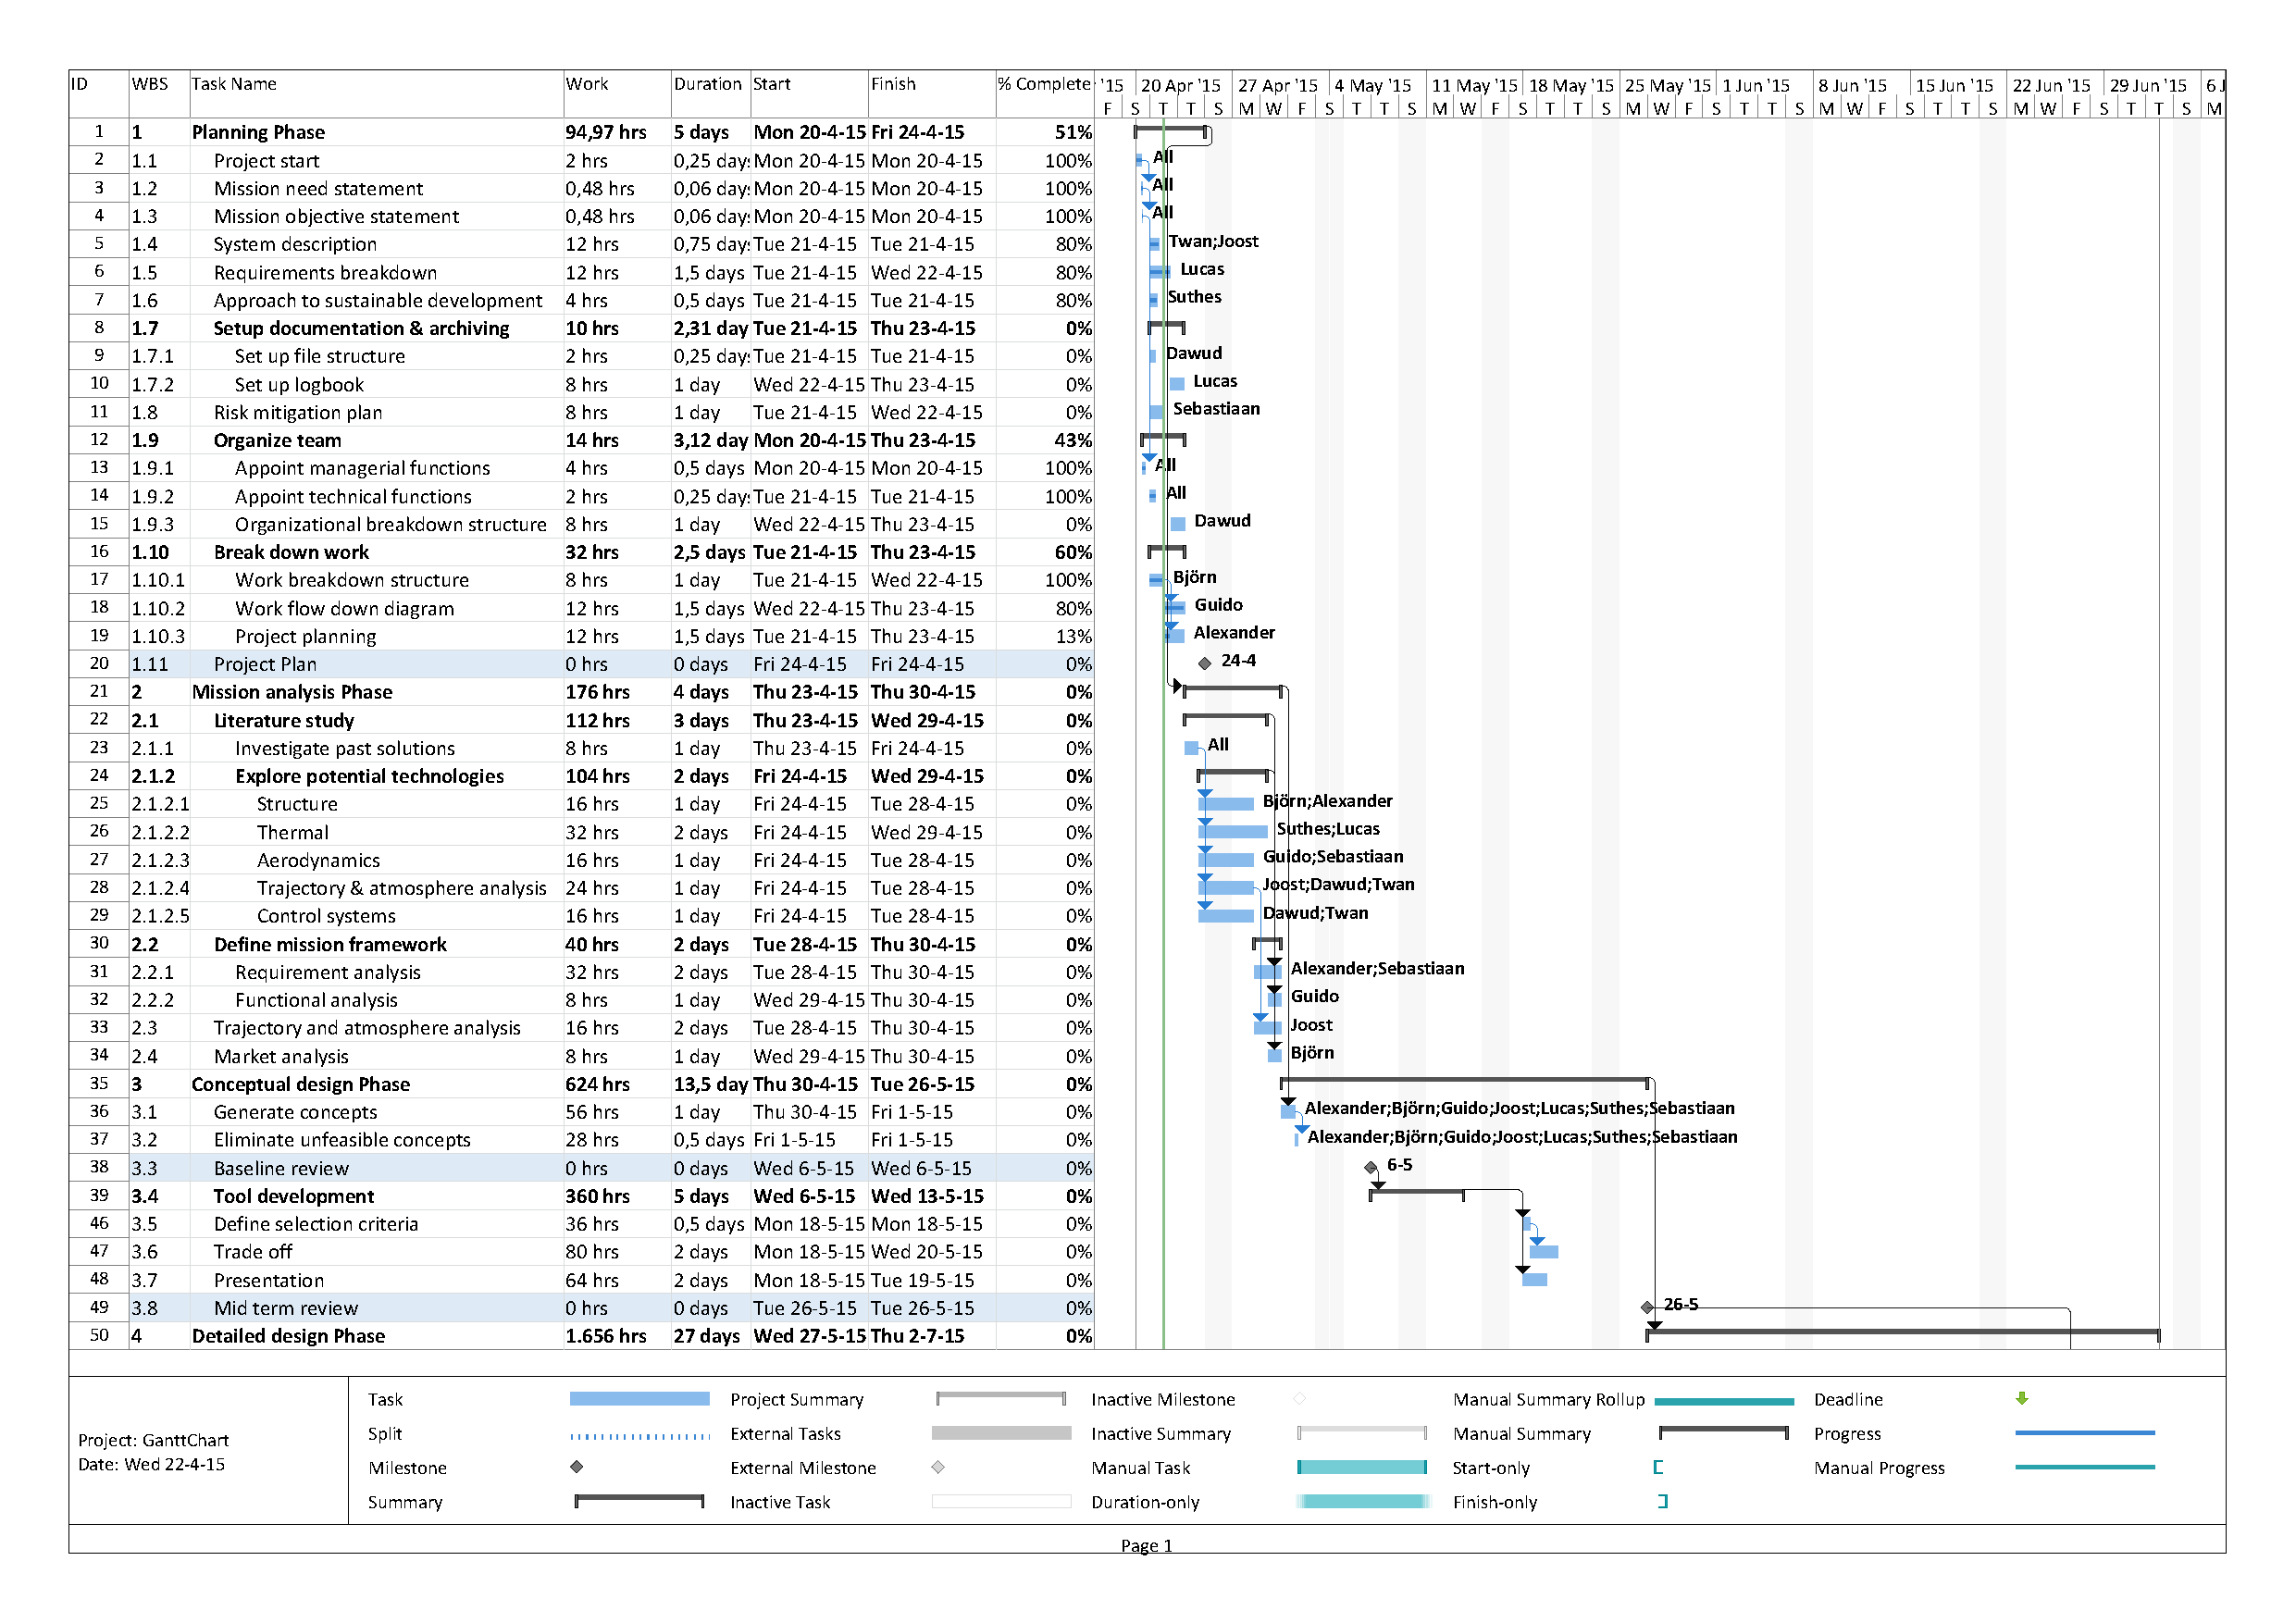
\includegraphics[scale=0.9]{Figure/GanttChart.pdf}
    \caption{Project planning}
    \label{fig:GanttChart}
\end{sidewaysfigure}

\begin{sidewaysfigure}[ht]
    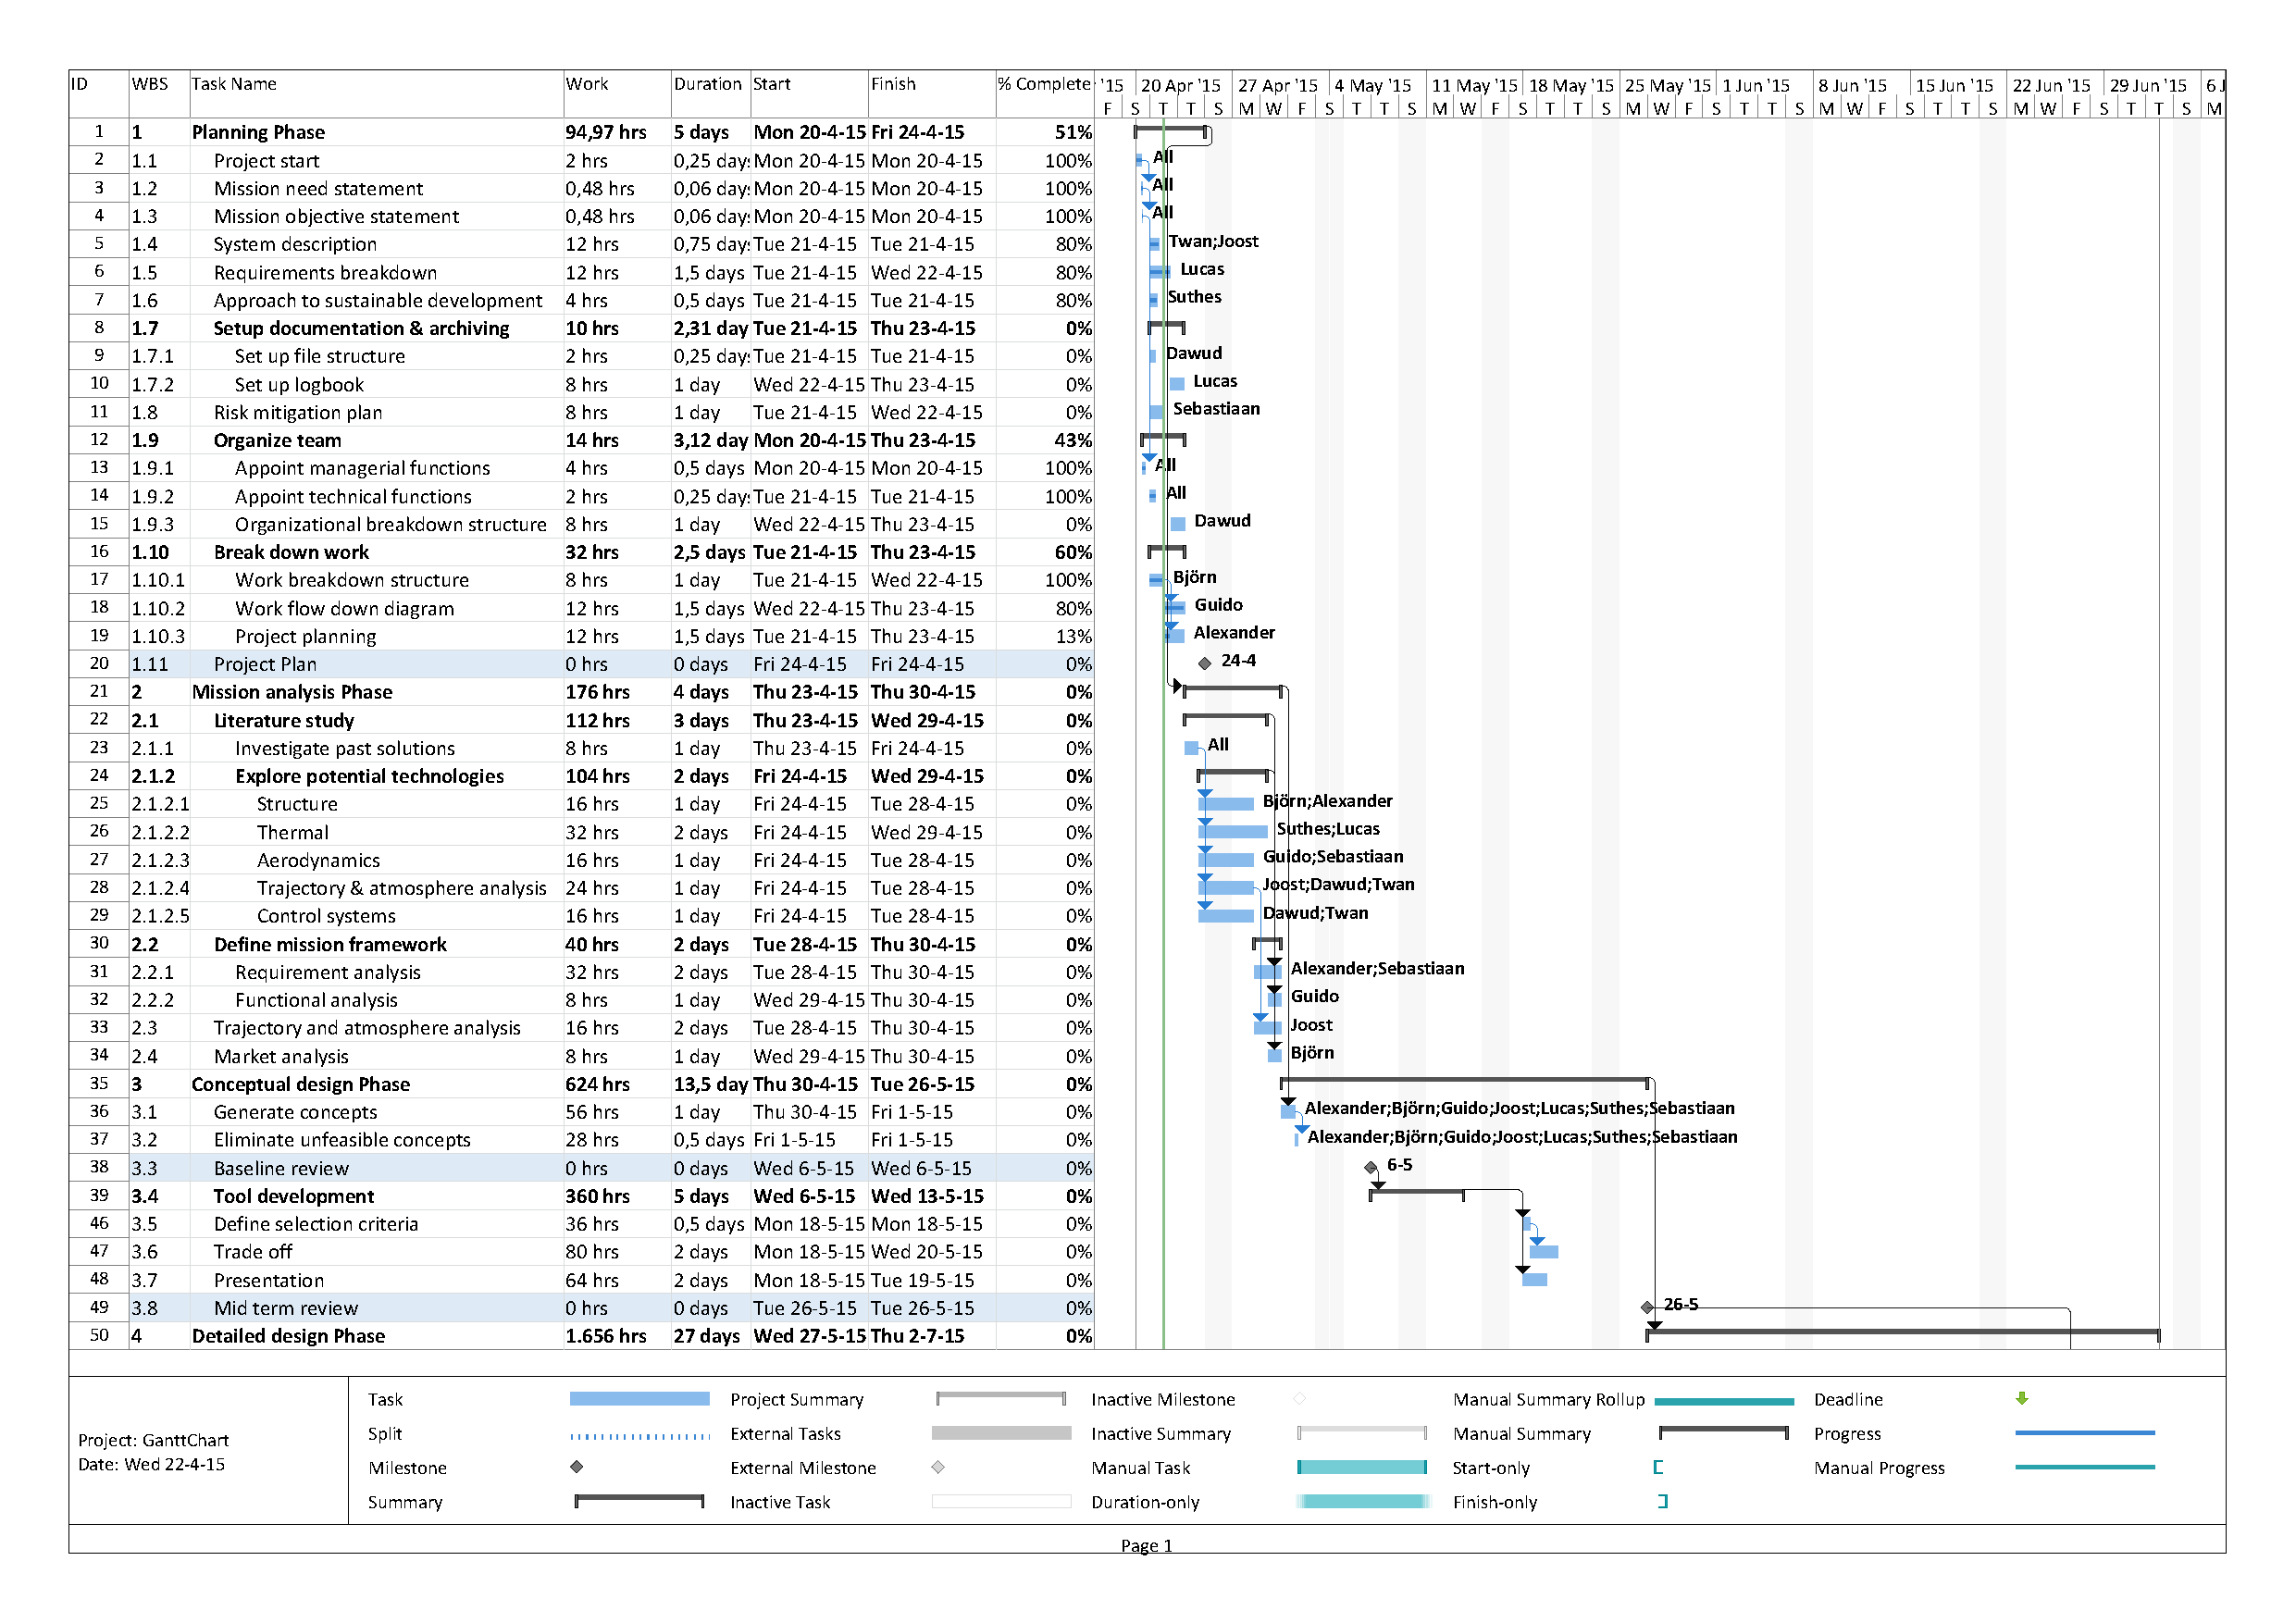
\includegraphics[scale=0.9]{Figure/GanttChart.pdf}
    \caption{Project planning}
\end{sidewaysfigure}

\end{document}